\documentclass[simplex.tex]{subfiles}
% DO NOT INCLUDE PREAMBLES/PACKAGES HERE!!
% packages are inherited from preamble.tex; you can compile this on its own
\begin{document}
\subsection{Multiscale Generalized Correlation (MGC)}

We developed the Multiscale Generalized Correlation method to better detect associations between two datasets $X$ and $Y$. We demonstrate that Oracle MGC is a consistent test statistic (power converge to 1 as sample size increases) under standard regularity conditions, is equivalently to the global correlation under linear dependency (i.e., each observation $X_i$ is a linear transformation of $Y_i$), and can be strictly better than the global correlation under common nonlinear dependencies. Thus Oracle MGC dominates the global correlation, and the sample MGC (i.e., choose the optimal scale by p-value map approximation, as the testing power are not available in the absence of the true model and training data) also empirically dominates the global correlation. The performance advantage of MGC is shown in Figure~\ref{fig:all}.
%
\begin{figure}[h!]
\begin{cframed}
		\centering
		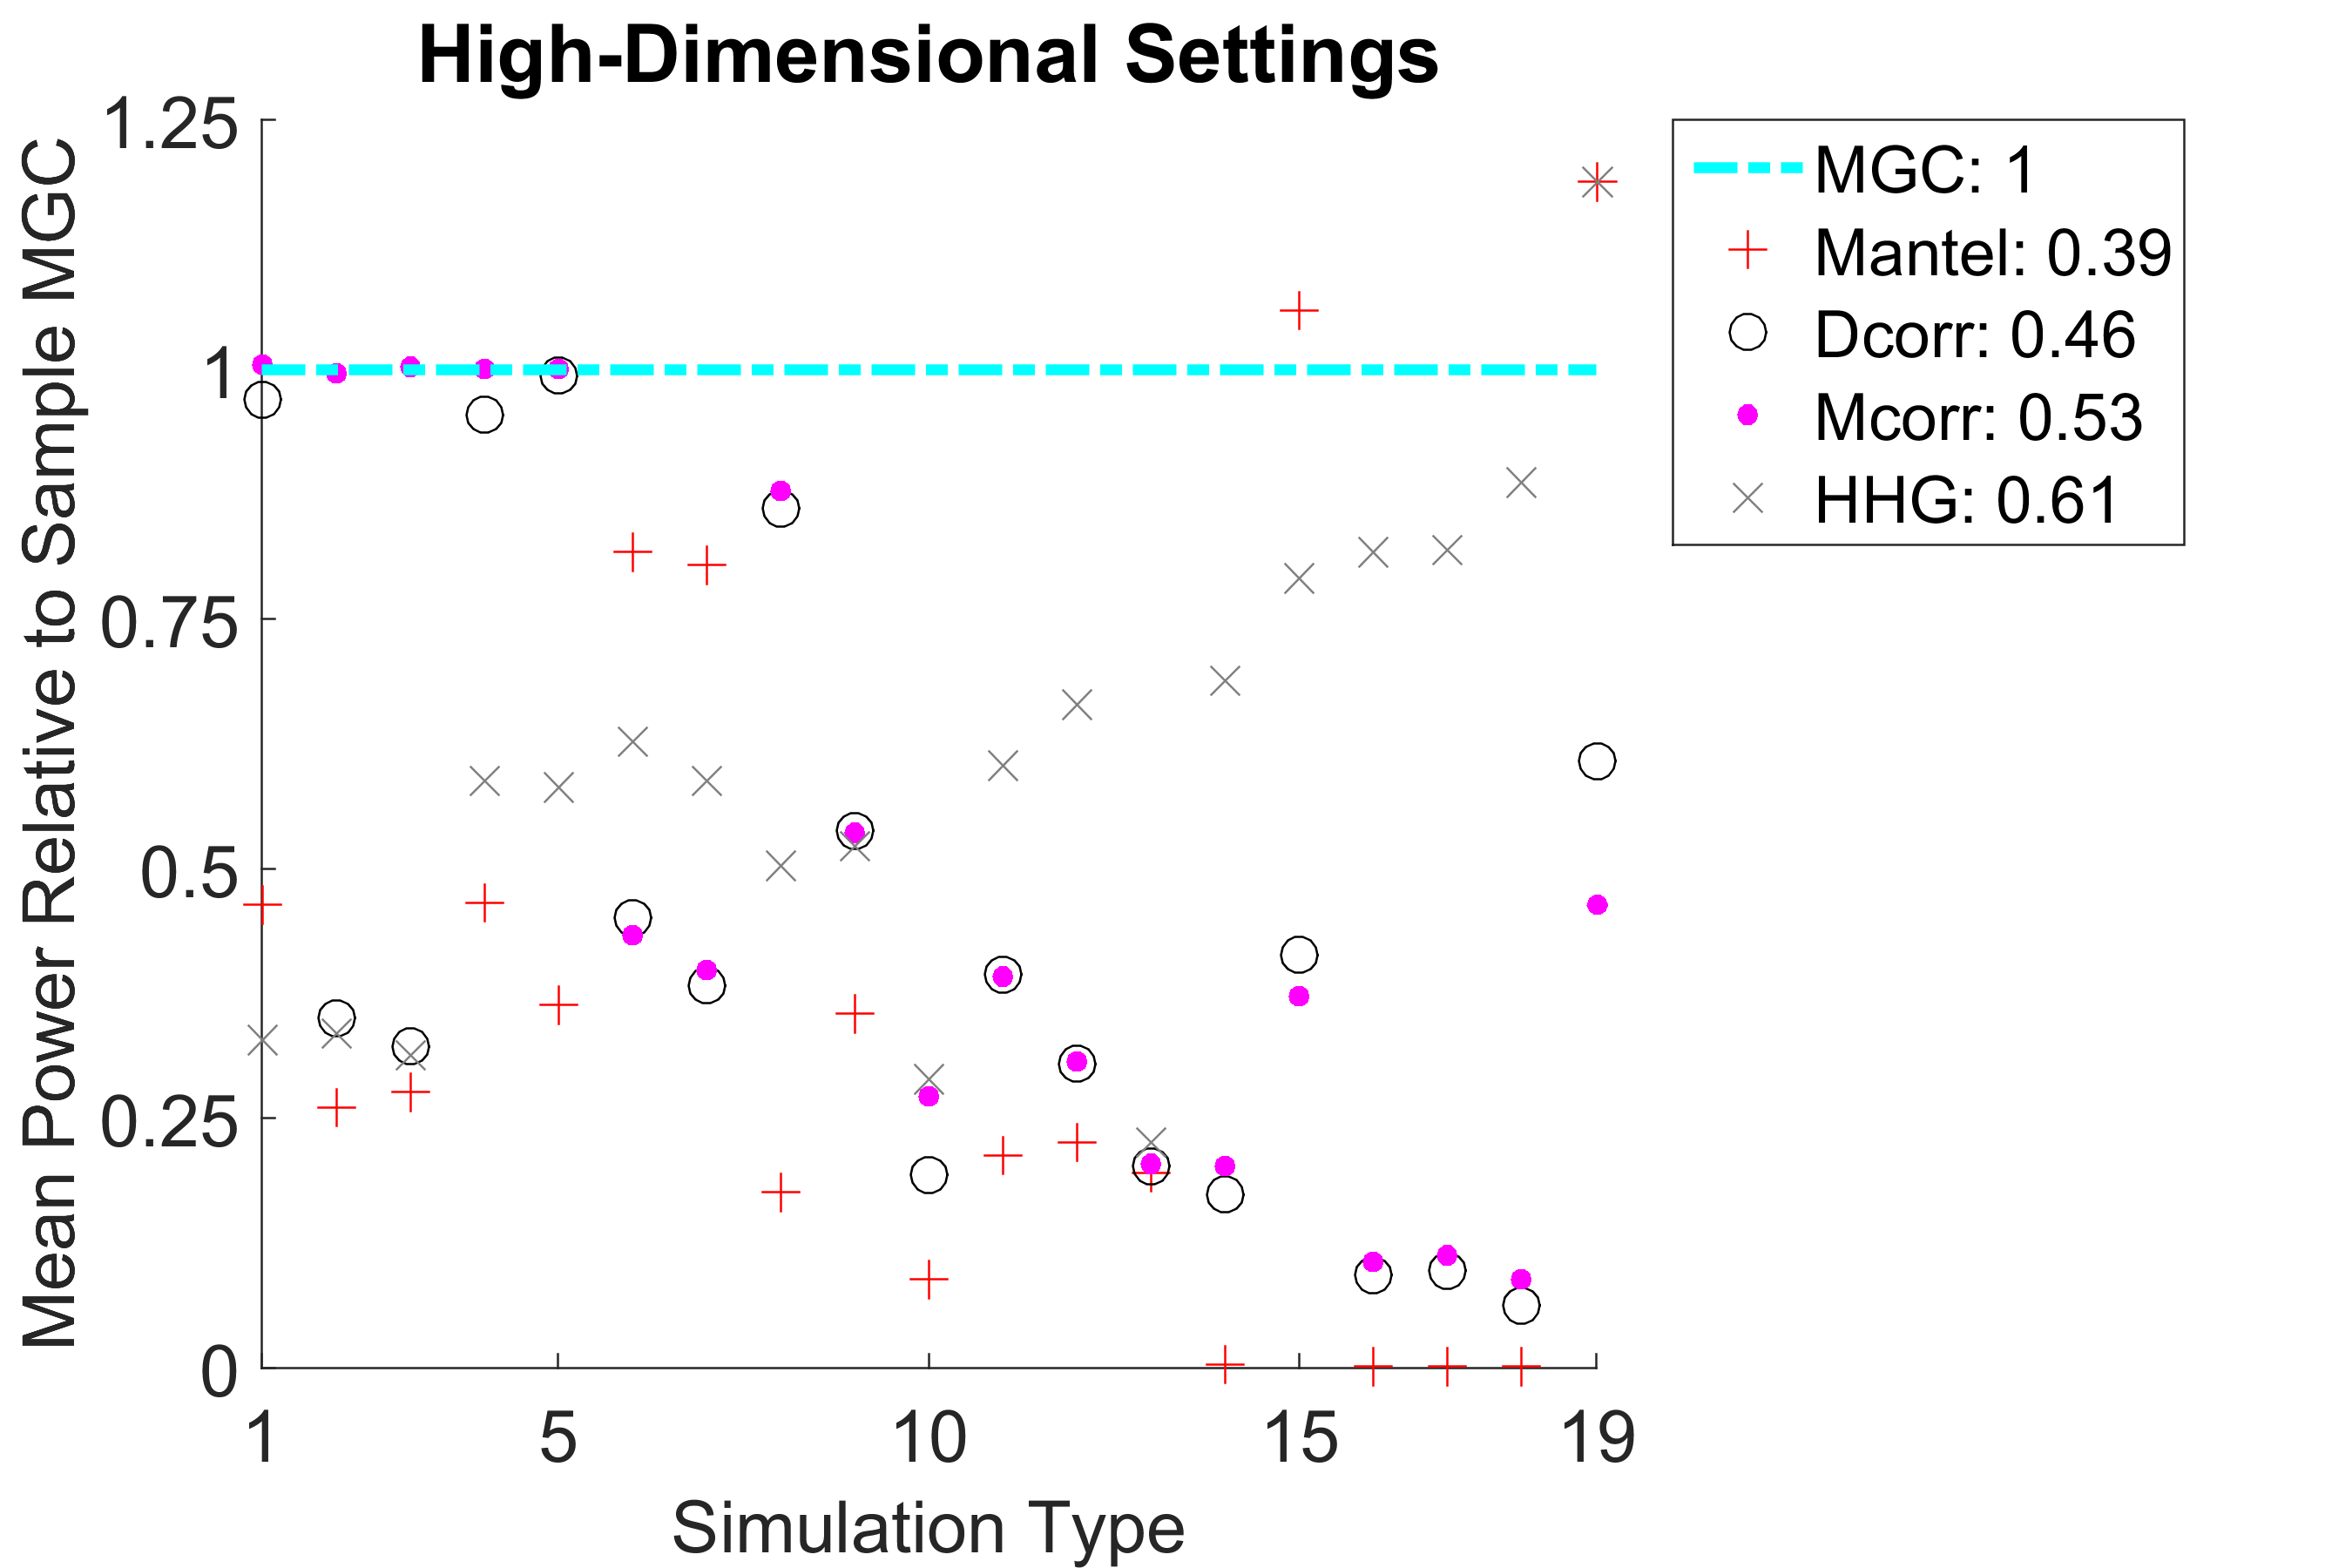
\includegraphics[width=0.8\textwidth]{../../figs/FigHDPowerSummary}
    \caption{The average power advantage of MGC versus popular benchmarks, throughout $20$ different linear and nonlinear high-dimensional dependencies.}
		\label{fig:all}
		\end{cframed}
\end{figure}

Upon final draft polishing and addressing feedback from statisticians and biologists, the newest draft is updated to \href{https://arxiv.org/pdf/1609.05148.pdf}{arXiv} and submitted for publication. 

\clearpage
\end{document}
